\PassOptionsToPackage{unicode=true}{hyperref} % options for packages loaded elsewhere
\PassOptionsToPackage{hyphens}{url}
%
\documentclass[]{book}
\usepackage{lmodern}
\usepackage{amssymb,amsmath}
\usepackage{ifxetex,ifluatex}
\usepackage{fixltx2e} % provides \textsubscript
\ifnum 0\ifxetex 1\fi\ifluatex 1\fi=0 % if pdftex
  \usepackage[T1]{fontenc}
  \usepackage[utf8]{inputenc}
  \usepackage{textcomp} % provides euro and other symbols
\else % if luatex or xelatex
  \usepackage{unicode-math}
  \defaultfontfeatures{Ligatures=TeX,Scale=MatchLowercase}
\fi
% use upquote if available, for straight quotes in verbatim environments
\IfFileExists{upquote.sty}{\usepackage{upquote}}{}
% use microtype if available
\IfFileExists{microtype.sty}{%
\usepackage[]{microtype}
\UseMicrotypeSet[protrusion]{basicmath} % disable protrusion for tt fonts
}{}
\IfFileExists{parskip.sty}{%
\usepackage{parskip}
}{% else
\setlength{\parindent}{0pt}
\setlength{\parskip}{6pt plus 2pt minus 1pt}
}
\usepackage{hyperref}
\hypersetup{
            pdftitle={Tools for Analyzing Data},
            pdfauthor={Nicole Sorhagen, Ph.D.},
            pdfborder={0 0 0},
            breaklinks=true}
\urlstyle{same}  % don't use monospace font for urls
\usepackage{longtable,booktabs}
% Fix footnotes in tables (requires footnote package)
\IfFileExists{footnote.sty}{\usepackage{footnote}\makesavenoteenv{longtable}}{}
\usepackage{graphicx,grffile}
\makeatletter
\def\maxwidth{\ifdim\Gin@nat@width>\linewidth\linewidth\else\Gin@nat@width\fi}
\def\maxheight{\ifdim\Gin@nat@height>\textheight\textheight\else\Gin@nat@height\fi}
\makeatother
% Scale images if necessary, so that they will not overflow the page
% margins by default, and it is still possible to overwrite the defaults
% using explicit options in \includegraphics[width, height, ...]{}
\setkeys{Gin}{width=\maxwidth,height=\maxheight,keepaspectratio}
\setlength{\emergencystretch}{3em}  % prevent overfull lines
\providecommand{\tightlist}{%
  \setlength{\itemsep}{0pt}\setlength{\parskip}{0pt}}
\setcounter{secnumdepth}{5}
% Redefines (sub)paragraphs to behave more like sections
\ifx\paragraph\undefined\else
\let\oldparagraph\paragraph
\renewcommand{\paragraph}[1]{\oldparagraph{#1}\mbox{}}
\fi
\ifx\subparagraph\undefined\else
\let\oldsubparagraph\subparagraph
\renewcommand{\subparagraph}[1]{\oldsubparagraph{#1}\mbox{}}
\fi

% set default figure placement to htbp
\makeatletter
\def\fps@figure{htbp}
\makeatother

\usepackage{booktabs}
\usepackage{amsthm}
\makeatletter
\def\thm@space@setup{%
  \thm@preskip=8pt plus 2pt minus 4pt
  \thm@postskip=\thm@preskip
}
\makeatother
\usepackage[]{natbib}
\bibliographystyle{apalike}

\title{Tools for Analyzing Data}
\author{Nicole Sorhagen, Ph.D.}
\date{2020-05-19}

\begin{document}
\maketitle

{
\setcounter{tocdepth}{1}
\tableofcontents
}
\hypertarget{about-this-book}{%
\chapter{About this book}\label{about-this-book}}

\hypertarget{introduction}{%
\chapter{Introduction}\label{introduction}}

\hypertarget{console}{%
\section{Console}\label{console}}

The console panel of R studio is where you can type commands and where you will see the output of commands.

In its most basic form, you can think of R as a fancy calculator.

For example:

In the console type \texttt{2+2} and then press \textbf{RETURN} on your keyboard.

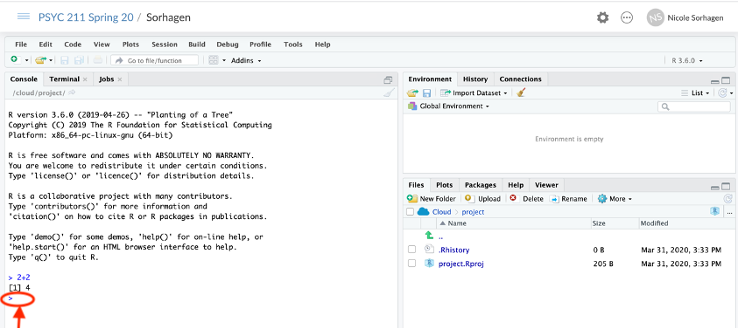
\includegraphics{img/twoplus.png}

Note that the \texttt{\textgreater{}} in the last line of the console means that the console is ready for a command (see red circle in the picture above). If \texttt{\textgreater{}} is missing from the last line, it means that R is waiting for you.

For example, type \texttt{1+} in the console and then hit enter.

The blinking cursor means that the command is incomplete.

Push the \textbf{ESC} button on your keyboard to get back to the command prompt.

\hypertarget{script}{%
\section{Script}\label{script}}

One of the benefits of using R is that you can save a record of your work using scripts. Records of your work allow you to easily start and stop an assignment or research project. You can pick up where you left off whether it is 20 minutes later or 2 years later. It also lets you share with others -- from professors, to collaborators, to peer reviewers.

To create a new script, go to the top bar menu:

\textbf{FILE -\textgreater{} NEW FILE -\textgreater{} R SCRIPT}

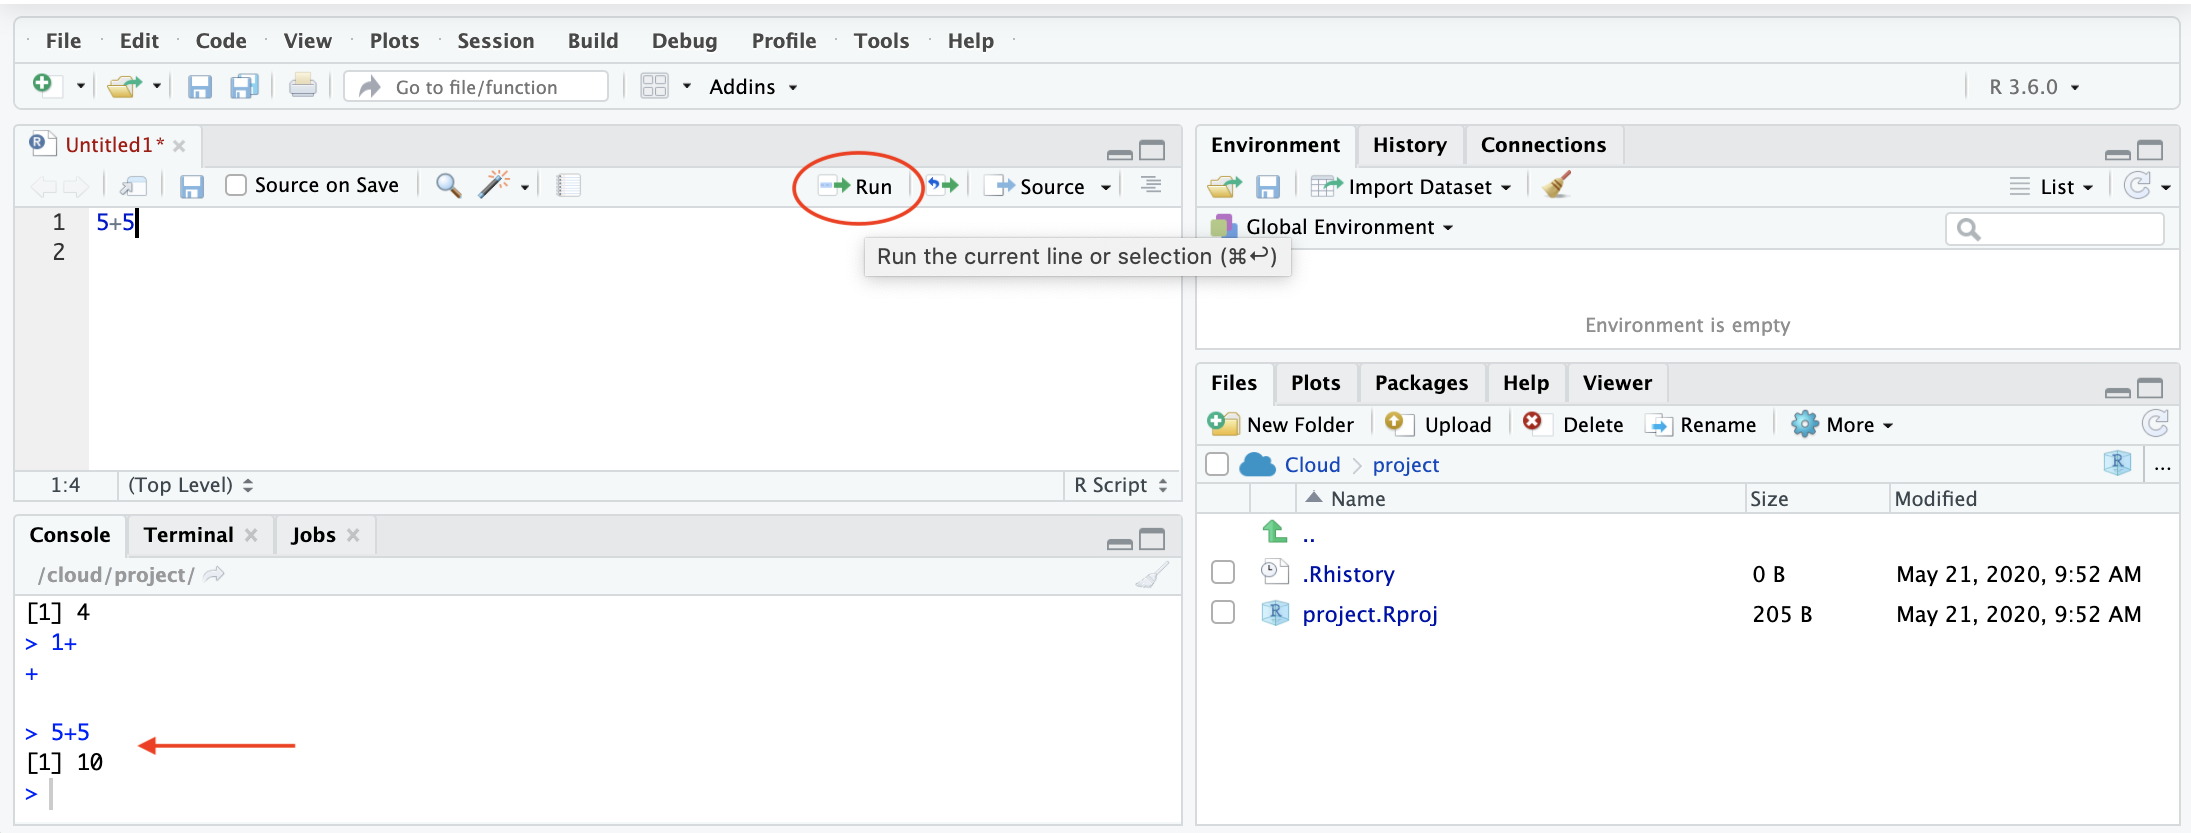
\includegraphics{img/script.png}

** You should run all code from a script **

Scripts are similar to running code in the console (this is what you did in the last section). For example, type `5+5' in the script panel.

In order to run code in a script you should click the run button while the cursor is in the code or the code is selected. You can also select the code and press the COMMAND and RETURN keys at the same time (the ALT and RETURN key on a pc).

ADD NEW PICTURE HERE AND NOTE THAT THE RESULTS WILL APPEAR AUTOMATICALLY IN THE CONSOLE

\hypertarget{environment-and-history}{%
\section{Environment and history}\label{environment-and-history}}

In the top right corner of RStudio is the environment and history window. The history tab shows every line of code that has been run in the current session.

The environment tab is where all active objects are listed. An object is something can hold information for later use. The information can be data, values, output, or functions. In this class we will store data and values in objects (we might get to storing output in an object in the last lab).

\hypertarget{set-up-project-on-rstudio-cloud}{%
\chapter{Set up project on Rstudio Cloud}\label{set-up-project-on-rstudio-cloud}}

First expand the R studio cloud options by clicking on the 3 lines in the top left corner.

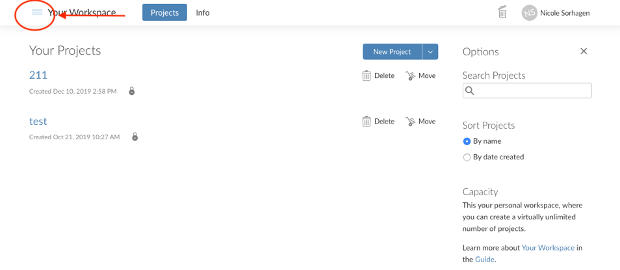
\includegraphics{img/Picture1.png}

Then select PSYC 211 for the current semester. If you cannot see this option -- then you have not been added to our shared workspace. See the Introduction to R -- overview (start here) html site on this week's D2L site for instructions on how to get into our shared workspace.

Once you are in the shared PSYC 211 workspace, open a new project and title it with your last name by clicking on the box that says `Untitled Project' and typing your last name.

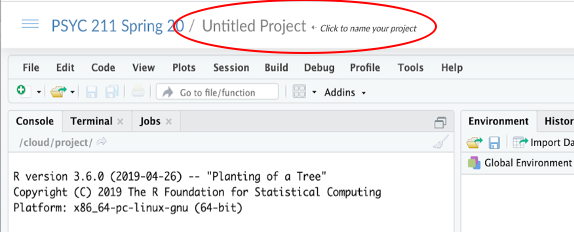
\includegraphics{img/Projname.png}

I will be able to see everyone's project. But you will only be able to see your project and my project.

\hypertarget{final-words}{%
\chapter{Final Words}\label{final-words}}

We have finished a nice book.

\bibliography{book.bib,packages.bib}

\end{document}
